% Options for packages loaded elsewhere
\PassOptionsToPackage{unicode}{hyperref}
\PassOptionsToPackage{hyphens}{url}
%
\documentclass[
]{book}
\usepackage{lmodern}
\usepackage{amsmath}
\usepackage{ifxetex,ifluatex}
\ifnum 0\ifxetex 1\fi\ifluatex 1\fi=0 % if pdftex
  \usepackage[T1]{fontenc}
  \usepackage[utf8]{inputenc}
  \usepackage{textcomp} % provide euro and other symbols
  \usepackage{amssymb}
\else % if luatex or xetex
  \usepackage{unicode-math}
  \defaultfontfeatures{Scale=MatchLowercase}
  \defaultfontfeatures[\rmfamily]{Ligatures=TeX,Scale=1}
\fi
% Use upquote if available, for straight quotes in verbatim environments
\IfFileExists{upquote.sty}{\usepackage{upquote}}{}
\IfFileExists{microtype.sty}{% use microtype if available
  \usepackage[]{microtype}
  \UseMicrotypeSet[protrusion]{basicmath} % disable protrusion for tt fonts
}{}
\makeatletter
\@ifundefined{KOMAClassName}{% if non-KOMA class
  \IfFileExists{parskip.sty}{%
    \usepackage{parskip}
  }{% else
    \setlength{\parindent}{0pt}
    \setlength{\parskip}{6pt plus 2pt minus 1pt}}
}{% if KOMA class
  \KOMAoptions{parskip=half}}
\makeatother
\usepackage{xcolor}
\IfFileExists{xurl.sty}{\usepackage{xurl}}{} % add URL line breaks if available
\IfFileExists{bookmark.sty}{\usepackage{bookmark}}{\usepackage{hyperref}}
\hypersetup{
  pdftitle={Bygge statistisk modeller med kategoriske variabler (ANOVA, t-test)},
  pdfauthor={Christian Magelssen},
  hidelinks,
  pdfcreator={LaTeX via pandoc}}
\urlstyle{same} % disable monospaced font for URLs
\usepackage{color}
\usepackage{fancyvrb}
\newcommand{\VerbBar}{|}
\newcommand{\VERB}{\Verb[commandchars=\\\{\}]}
\DefineVerbatimEnvironment{Highlighting}{Verbatim}{commandchars=\\\{\}}
% Add ',fontsize=\small' for more characters per line
\usepackage{framed}
\definecolor{shadecolor}{RGB}{248,248,248}
\newenvironment{Shaded}{\begin{snugshade}}{\end{snugshade}}
\newcommand{\AlertTok}[1]{\textcolor[rgb]{0.94,0.16,0.16}{#1}}
\newcommand{\AnnotationTok}[1]{\textcolor[rgb]{0.56,0.35,0.01}{\textbf{\textit{#1}}}}
\newcommand{\AttributeTok}[1]{\textcolor[rgb]{0.77,0.63,0.00}{#1}}
\newcommand{\BaseNTok}[1]{\textcolor[rgb]{0.00,0.00,0.81}{#1}}
\newcommand{\BuiltInTok}[1]{#1}
\newcommand{\CharTok}[1]{\textcolor[rgb]{0.31,0.60,0.02}{#1}}
\newcommand{\CommentTok}[1]{\textcolor[rgb]{0.56,0.35,0.01}{\textit{#1}}}
\newcommand{\CommentVarTok}[1]{\textcolor[rgb]{0.56,0.35,0.01}{\textbf{\textit{#1}}}}
\newcommand{\ConstantTok}[1]{\textcolor[rgb]{0.00,0.00,0.00}{#1}}
\newcommand{\ControlFlowTok}[1]{\textcolor[rgb]{0.13,0.29,0.53}{\textbf{#1}}}
\newcommand{\DataTypeTok}[1]{\textcolor[rgb]{0.13,0.29,0.53}{#1}}
\newcommand{\DecValTok}[1]{\textcolor[rgb]{0.00,0.00,0.81}{#1}}
\newcommand{\DocumentationTok}[1]{\textcolor[rgb]{0.56,0.35,0.01}{\textbf{\textit{#1}}}}
\newcommand{\ErrorTok}[1]{\textcolor[rgb]{0.64,0.00,0.00}{\textbf{#1}}}
\newcommand{\ExtensionTok}[1]{#1}
\newcommand{\FloatTok}[1]{\textcolor[rgb]{0.00,0.00,0.81}{#1}}
\newcommand{\FunctionTok}[1]{\textcolor[rgb]{0.00,0.00,0.00}{#1}}
\newcommand{\ImportTok}[1]{#1}
\newcommand{\InformationTok}[1]{\textcolor[rgb]{0.56,0.35,0.01}{\textbf{\textit{#1}}}}
\newcommand{\KeywordTok}[1]{\textcolor[rgb]{0.13,0.29,0.53}{\textbf{#1}}}
\newcommand{\NormalTok}[1]{#1}
\newcommand{\OperatorTok}[1]{\textcolor[rgb]{0.81,0.36,0.00}{\textbf{#1}}}
\newcommand{\OtherTok}[1]{\textcolor[rgb]{0.56,0.35,0.01}{#1}}
\newcommand{\PreprocessorTok}[1]{\textcolor[rgb]{0.56,0.35,0.01}{\textit{#1}}}
\newcommand{\RegionMarkerTok}[1]{#1}
\newcommand{\SpecialCharTok}[1]{\textcolor[rgb]{0.00,0.00,0.00}{#1}}
\newcommand{\SpecialStringTok}[1]{\textcolor[rgb]{0.31,0.60,0.02}{#1}}
\newcommand{\StringTok}[1]{\textcolor[rgb]{0.31,0.60,0.02}{#1}}
\newcommand{\VariableTok}[1]{\textcolor[rgb]{0.00,0.00,0.00}{#1}}
\newcommand{\VerbatimStringTok}[1]{\textcolor[rgb]{0.31,0.60,0.02}{#1}}
\newcommand{\WarningTok}[1]{\textcolor[rgb]{0.56,0.35,0.01}{\textbf{\textit{#1}}}}
\usepackage{longtable,booktabs}
\usepackage{calc} % for calculating minipage widths
% Correct order of tables after \paragraph or \subparagraph
\usepackage{etoolbox}
\makeatletter
\patchcmd\longtable{\par}{\if@noskipsec\mbox{}\fi\par}{}{}
\makeatother
% Allow footnotes in longtable head/foot
\IfFileExists{footnotehyper.sty}{\usepackage{footnotehyper}}{\usepackage{footnote}}
\makesavenoteenv{longtable}
\usepackage{graphicx}
\makeatletter
\def\maxwidth{\ifdim\Gin@nat@width>\linewidth\linewidth\else\Gin@nat@width\fi}
\def\maxheight{\ifdim\Gin@nat@height>\textheight\textheight\else\Gin@nat@height\fi}
\makeatother
% Scale images if necessary, so that they will not overflow the page
% margins by default, and it is still possible to overwrite the defaults
% using explicit options in \includegraphics[width, height, ...]{}
\setkeys{Gin}{width=\maxwidth,height=\maxheight,keepaspectratio}
% Set default figure placement to htbp
\makeatletter
\def\fps@figure{htbp}
\makeatother
\setlength{\emergencystretch}{3em} % prevent overfull lines
\providecommand{\tightlist}{%
  \setlength{\itemsep}{0pt}\setlength{\parskip}{0pt}}
\setcounter{secnumdepth}{5}
\usepackage{booktabs}

\newenvironment{danger}
    {
    \hline\\
    }
    { 
    \\\\\hline
    }
    
\newenvironment{warning}
    {
    \hline\\
    }
    { 
    \\\\\hline
    }
    
\newenvironment{info}
    {
    \hline\\
    }
    { 
    \\\\\hline
    }
    
\newenvironment{try}
    {
    \hline\\
    }
    { 
    \\\\\hline
    }
\ifluatex
  \usepackage{selnolig}  % disable illegal ligatures
\fi
\usepackage[]{natbib}
\bibliographystyle{apalike}

\title{Bygge statistisk modeller med kategoriske variabler (ANOVA, t-test)}
\author{Christian Magelssen}
\date{2021-04-05}

\begin{document}
\maketitle

{
\setcounter{tocdepth}{1}
\tableofcontents
}
\hypertarget{intro}{%
\chapter{Introduksjon}\label{intro}}

I dette kapittelet skal vi lære å bygge statistiske modeller for å teste om \textbf{to eller flere grupper er forskjellige på en avhengig variabel som er kontinuerlig}.

En variabel kan sies å være \textbf{kontinuerlig} når vi kan bestemme hvor presist vi ønsker å måle den. For eksempel regnes tid som en kontuerlig variabel fordi det (i prinsippet) ikke finnes noen grenser hvor presist vi kan måle tid; vi kan måle det i år, måneder, uker, dager, timer, minutter, sekunder, tideler, hundredeler eller tusendeler.

\textbf{Grupper} defineres i psykologifaget som en samling mennesker som deler bestemte karakterstikker. Det kan være spillere på et fotballag, individer på et treningssenter, eller menn og kvinner. Dette er også eksempler på naturlig inndelte grupper i samfunnet. Noen ganger kan det være interessant å se om disse gruppene er forskjellige. For eksempel kan det være interessant å se om individer som trener på treningssenter er sterkere enn de som ikke trener på treningssenter.

Andre ganger kan det være interessant å teste om to grupper, som var like før et eksperiment, har blitt forskjellige fordi vi har behandlet dem ulikt. Vi randomiserer individer i to ulike grupper, slik at vi sikrer at vi blander disse individene godt (f.eks kjønn, motivasjon, interesser). Hvis eksperimentet har blitt gjennomført godt at det ikke er noen andre forklaringer på at disse to gruppene har blitt forskjellige etter intervensjonsperioden, så kan vi trekke en slutning om disse to gruppene trolig ikke kommer fra samme populasjon lenger; eksperimentet har gjort at disse to gruppene trolig kommer fra to forskjellige populasjoner.

\hypertarget{om-denne-boken}{%
\section{Om denne boken}\label{om-denne-boken}}

Denne boken er skrevet i R.

\hypertarget{datasett}{%
\chapter{Datasett}\label{datasett}}

\hypertarget{buxf8r-man-trene-med-ett-eller-flere-sett-i-styrketrening}{%
\section{Bør man trene med ett eller flere sett i styrketrening?}\label{buxf8r-man-trene-med-ett-eller-flere-sett-i-styrketrening}}

Mange utrente lurer på hvor mange serier de bør gjennnomføre for å oppnå maksimal treningseffekt i styrketrening. Noen føler at de blir slitne etter ett sett og at dette derfor er tilstrekkelig. Andre mener at et hardere treningstimuli er nødvendig, selv om man er utrent, og at to eller flere sett derfor er bedre. En forsker som var tidlig ute med å undersøke var Bent Rønnestad \citep{ronnestad_dissimilar_2007}

Eksperimentet ble gjennomført som et \textbf{between-subject design} med to grupper:
* en gruppe trente 1 sett på underkroppen og 3 sett på overkroppen
* en annen gruppe trente 3 sett på underkroppen og 1 sett på overkroppen.

Disse gruppene kalte han henholdsvis \textbf{1L-3U} og \textbf{3L-1U} (L=lower; U=Upper).

De to gruppene trente 3 ganger i uken i totalt 11 uker. Forskergruppen ville så se hva som ga mest fremgang i 1RM på underkroppsøvelser. Den avhengige variabelen ble derfor \%-fremgang på 1RM på underkroppsøvelser.

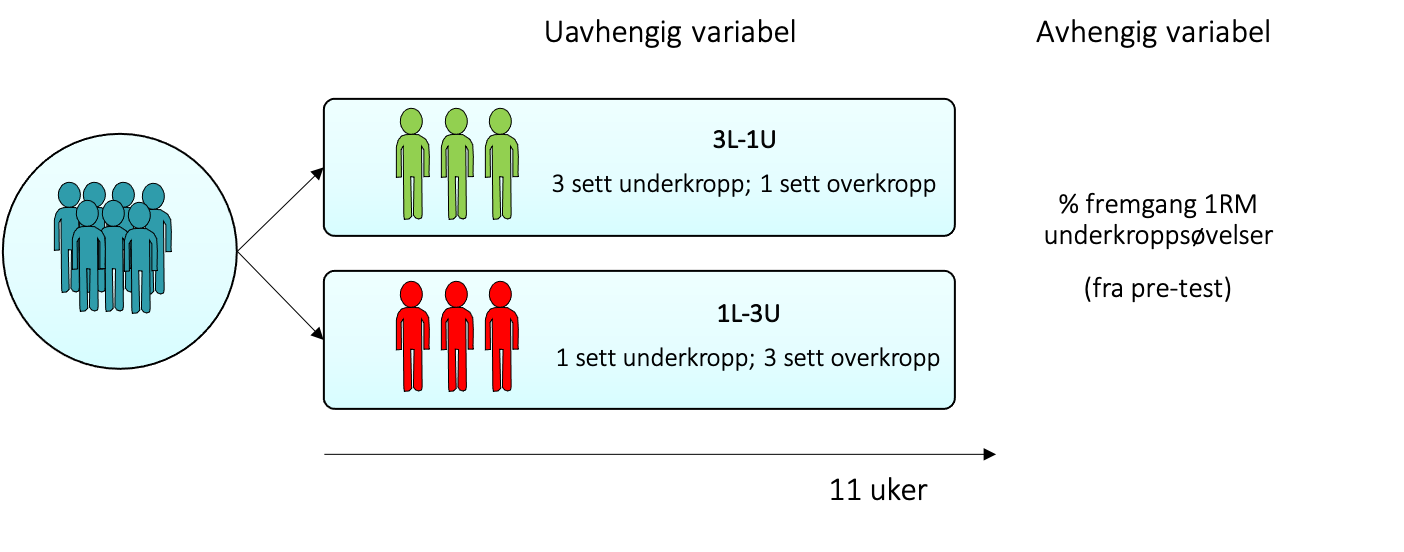
\includegraphics{design.png}
Vi har ikke tilgang til dette datasettet, men vi har simulert dette datasettet i R basert på verdiene som ble oppgitt i artikkelen. Datasettet blir tilnærmet likt, men siden det er en simulering blir det aldri helt identisk. Datasettet ser du i tabellen under.

\begin{table}

\caption{\label{tab:unnamed-chunk-3}Simulert datasett}
\centering
\begin{tabular}[t]{rlr}
\toprule
individ & gruppe & rm\\
\midrule
1 & tre.sett & 40.46704\\
2 & tre.sett & 49.07223\\
3 & tre.sett & 47.94131\\
4 & tre.sett & 44.51389\\
5 & tre.sett & 52.28750\\
\addlinespace
6 & tre.sett & 40.01750\\
7 & tre.sett & 49.48425\\
8 & tre.sett & 29.21048\\
9 & tre.sett & 40.59293\\
10 & tre.sett & 37.58676\\
\addlinespace
11 & tre.sett & 35.42651\\
12 & tre.sett & 42.49354\\
13 & ett.sett & 17.70576\\
14 & ett.sett & 17.07181\\
15 & ett.sett & 18.26811\\
\addlinespace
16 & ett.sett & 25.42594\\
17 & ett.sett & 32.70313\\
18 & ett.sett & 19.10226\\
19 & ett.sett & 22.23827\\
20 & ett.sett & 22.27148\\
\addlinespace
21 & ett.sett & 26.17889\\
22 & ett.sett & 20.34857\\
23 & ett.sett & 23.52773\\
24 & ett.sett & 17.95966\\
\bottomrule
\end{tabular}
\end{table}

Du kan få nøyaktig samme datsett ved å klippe ut og lime inn følgende kode i en skript-fil i R (husk å laste inn tidyverse-pakken, library(tidyverse) ). Du kan også laste ned datasettet som en .csv fil fra canvas.

\begin{Shaded}
\begin{Highlighting}[]
\FunctionTok{set.seed}\NormalTok{(}\DecValTok{2002}\NormalTok{) }\CommentTok{\#viktig å ha med denne for å få nøyaktig samme datasett}
\NormalTok{tre.sett }\OtherTok{\textless{}{-}} \FunctionTok{rnorm}\NormalTok{(}\AttributeTok{n =} \DecValTok{12}\NormalTok{, }\AttributeTok{mean =} \DecValTok{41}\NormalTok{, }\AttributeTok{sd =} \DecValTok{5}\NormalTok{) }\CommentTok{\#12 individer}
\NormalTok{ett.sett }\OtherTok{\textless{}{-}}\FunctionTok{rnorm}\NormalTok{(}\AttributeTok{n =} \DecValTok{12}\NormalTok{, }\AttributeTok{mean =} \DecValTok{21}\NormalTok{, }\AttributeTok{sd =} \DecValTok{5}\NormalTok{) }\CommentTok{\#12 individer}

\CommentTok{\#lager en tibble fra tidyverse{-}pakken. Må ha lastet inn tidyverse library(tidyverse) i scriptfilen}
\NormalTok{dat }\OtherTok{\textless{}{-}} \FunctionTok{tibble}\NormalTok{(}\AttributeTok{individ =} \FunctionTok{seq}\NormalTok{(}\DecValTok{1}\SpecialCharTok{:}\DecValTok{24}\NormalTok{),}
              \AttributeTok{gruppe =} \FunctionTok{rep}\NormalTok{(}\FunctionTok{c}\NormalTok{(}\StringTok{"tre.sett "}\NormalTok{, }\StringTok{"ett.sett"}\NormalTok{), }\FunctionTok{c}\NormalTok{(}\FunctionTok{length}\NormalTok{(tre.sett), }\FunctionTok{length}\NormalTok{(ett.sett))),}
              \AttributeTok{rm =} \FunctionTok{c}\NormalTok{(tre.sett , ett.sett))}
\end{Highlighting}
\end{Shaded}

{Oppgave}

Før du går videre er det greit at du gjør deg kjent med datasettet som vi har generert. Studer datasettet og svar på følgende spørsmål:

\begin{enumerate}
\def\labelenumi{\alph{enumi})}
\tightlist
\item
  Hvor mange kolonner er det i tabellen over?
\item
  Hvor mange deltakere var med i studien?
\item
  Hvilke to verdier har variabelen `\emph{gruppe}'? og
\end{enumerate}

\hypertarget{gjennomsnitt-for-de-to-gruppene}{%
\section{Gjennomsnitt for de to gruppene}\label{gjennomsnitt-for-de-to-gruppene}}

Bra! Det er alltid viktig å bli kjent med sitt eget datasett, men nå som du har det kan vi gå videre. Vi er interessert i om det er forskjeller mellom de to gruppene (``tre.sett'' vs.~ett.sett) på \% fremgang fra pre- til post-test. Så kanskje vi kan starte med å se om det er forskjeller i gjennomsnitt mellom to gruppene? Dette kan enkelt gjøres i R, Jamovi eller excel. Her er en kode for å løse dette i R:

\begin{Shaded}
\begin{Highlighting}[]
\CommentTok{\#jeg lager et oobjekt som heter mean\_rm }
\NormalTok{mean\_rm }\OtherTok{\textless{}{-}}\NormalTok{ dat }\SpecialCharTok{\%\textgreater{}\%}
  \CommentTok{\#Jeg grupperer etter gruppe, slik at jeg får et mean for hver gruppe istf. for å få mean for alle individene}
  \CommentTok{\#group\_by er en funksjon for dette}
  \FunctionTok{group\_by}\NormalTok{(gruppe) }\SpecialCharTok{\%\textgreater{}\%}
  \CommentTok{\#deretter bruker jeg summarise funksjonen for å regne gjennomsnitt}
  \FunctionTok{summarise}\NormalTok{(}\AttributeTok{mean.fremgang.1RM =} \FunctionTok{mean}\NormalTok{(rm))}
\end{Highlighting}
\end{Shaded}

Koden gir oss følgende tabell:
\textbackslash begin\{table\}

\textbackslash caption\{\label{tab:unnamed-chunk-6}Gjennomsnittlige \%-vis fremgang for de to gruppene\}
\centering

\begin{tabular}[t]{lr}
\toprule
gruppe & mean.fremgang.1RM\\
\midrule
ett.sett & 21.90013\\
tre.sett & 42.42450\\
\bottomrule
\end{tabular}

\textbackslash end\{table\}

{Oppgave}

\begin{enumerate}
\def\labelenumi{\alph{enumi})}
\tightlist
\item
  Hvilken gruppe hadde mest fremgang?
  ett.sett tre.sett`
\end{enumerate}

\hypertarget{figur-av-datasettet}{%
\section{Figur av datasettet}\label{figur-av-datasettet}}

Vi kan også presentere dataen i en figur. For denne typen data er det veldig vanlig å bruke et \textbf{stolpediagram}:

\begin{figure}

{\centering 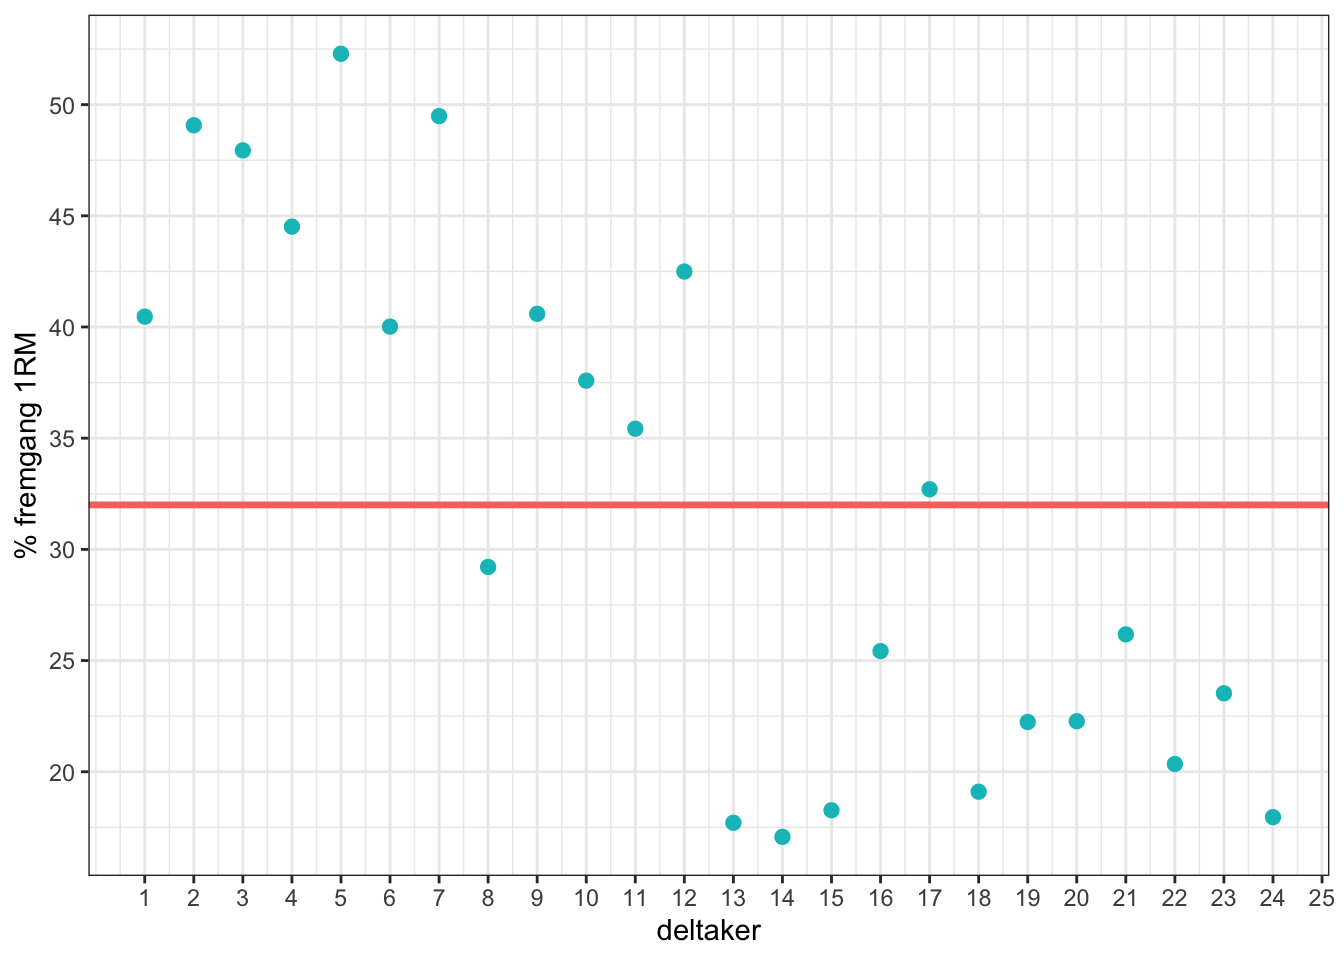
\includegraphics[width=0.6\linewidth]{02-datasett_files/figure-latex/unnamed-chunk-7-1} 

}

\caption{Modeller med forskjellig b1}\label{fig:unnamed-chunk-7}
\end{figure}

Et stolpediagram er pent å se på, men er egentlig designet for å kategoriske data. For eksempel er det fint å bruke dette når vi skal presentere frekvensen antall som har kjørt bil til skolen og antall personer som har gått. Les \citep{weissgerber_beyond_2015}(\url{https://journals.plos.org/plosbiology/article?id=10.1371/journal.pbio.1002128}). Deretter svar på følgende spørsmål for å se om du har forstått problemene ved å bruke stolpediagram på kontinuerlig data.

{Oppgave}

\begin{enumerate}
\def\labelenumi{\alph{enumi}.}
\item
  Stolpediagram er designet for kontinuerlig kategorisk data.
\item
  Høyden på stolpen representerer (bruk det norske begrepet!), hvilket vil si at det også må ligge noen observasjoner over og under stolpen.
\item
  Et stolpediagram viser ikke standard error standardavvik CI fordelingen av observasjonene, og dette spesielt være problematisk ved store små.
\item
  Forfatterne av artikkelen anbefaler mer bruk av bar graph scatterplot for kontinuerlige variabler.
\item
  Er standard error og standardavvik det samme? ja nei.
\end{enumerate}

\hypertarget{koding-av-kategoriske-prediktorvariabler}{%
\chapter{Koding av kategoriske prediktorvariabler}\label{koding-av-kategoriske-prediktorvariabler}}

I tabellen på forrige kan du se at vi har en tabell med tre kolonner: en kolonne for hver variabel vi har i vårt datasett.

\begin{itemize}
\tightlist
\item
  Variabelen \textbf{gruppe} er en kategorisk vaiabel som har to ulike verdier: ``ett.sett'' og ``tre.sett''. Dette er de to gruppene som vi skal teste om er forskjellige. I programmeringsverdenen kalles dette for et tekstobjekt, en string eller character. Uansett navn er problemet at vi ikke kan legge ord inn i en statistisk modell. Vi er nødt til å omkode den kategoriske variabelen med tallverdier. Det er flere måter å gjøre dette på, og måten man gjør det på har stor betydning for outfallet av den statistiske analysen.
\end{itemize}

De forskjellige måtene å kode kategoriske prediktorvariabler gir forskjellige resultater. En veldig vanlig måte å gjøre dette på er å bruke \textbf{dummykoding}. Dette kan fungere godt når du bygger enkle statistisk modeller, slik vi skal gjøre nå. Men dummykoding fungerer dårlig når du har mange grupper du ønsker å sammenligne, og du ikke ønsker å sammenligne disse gruppene mot en baseline gruppe. Da vil \textbf{kontrastkoding} være bedre egnet.

SPSS, R, Jamovi bruker dummykoding som standard, og det er viktig når du tolker resultatene fra modellene.

\hypertarget{dummykoding}{%
\section{Dummykoding}\label{dummykoding}}

En vanlig metode kalles \textbf{dummykoding} eller \textbf{treatment-koding}. Den går ut på å lage en eller flere variabler med 0 og 1 som de to mulige verdiene. Antall variabler vi trenger avhenger av antall grupper vi vil sammenligne. Siden vårt datasett kun inneholder to grupper, så trenger vi kun en variabel. Vi kan den ene gruppen og den andre 1. Hovedregelen er at vi gir 0 til baselinegruppe og 1 til den eksperimentelle gruppen. Vi gir derfor 0 til 1.sett-gruppen og 1 til 3.sett-gruppen. Gjør dette før du går videre.

I R og Jamovi kan du gjøre det med følgende if/else statement. I R kan du bruke følgende kode:

\begin{Shaded}
\begin{Highlighting}[]
\CommentTok{\#lager et nytt objekt som heter dummykodet.dat}
\NormalTok{dummykodet.dat }\OtherTok{\textless{}{-}}\NormalTok{ dat }\SpecialCharTok{\%\textgreater{}\%}
  \CommentTok{\# her lager jeg en ny kolonne som heter dummykoder. If gruppe == \textquotesingle{}ett.sett\textquotesingle{}, gi verdien 0, else gi de 1.}
  \FunctionTok{mutate}\NormalTok{(}\AttributeTok{dummykodet =} \FunctionTok{if\_else}\NormalTok{(gruppe }\SpecialCharTok{==} \StringTok{"ett.sett"}\NormalTok{, }\DecValTok{0}\NormalTok{, }\DecValTok{1}\NormalTok{))}
\end{Highlighting}
\end{Shaded}

\begin{table}

\caption{\label{tab:unnamed-chunk-4}Dummykodet datasett}
\centering
\begin{tabular}[t]{rlrr}
\toprule
individ & gruppe & rm & dummykodet\\
\midrule
1 & tre.sett & 40.46704 & 1\\
2 & tre.sett & 49.07223 & 1\\
3 & tre.sett & 47.94131 & 1\\
4 & tre.sett & 44.51389 & 1\\
5 & tre.sett & 52.28750 & 1\\
\addlinespace
6 & tre.sett & 40.01750 & 1\\
7 & tre.sett & 49.48425 & 1\\
8 & tre.sett & 29.21048 & 1\\
9 & tre.sett & 40.59293 & 1\\
10 & tre.sett & 37.58676 & 1\\
\addlinespace
11 & tre.sett & 35.42651 & 1\\
12 & tre.sett & 42.49354 & 1\\
13 & ett.sett & 17.70576 & 0\\
14 & ett.sett & 17.07181 & 0\\
15 & ett.sett & 18.26811 & 0\\
\addlinespace
16 & ett.sett & 25.42594 & 0\\
17 & ett.sett & 32.70313 & 0\\
18 & ett.sett & 19.10226 & 0\\
19 & ett.sett & 22.23827 & 0\\
20 & ett.sett & 22.27148 & 0\\
\addlinespace
21 & ett.sett & 26.17889 & 0\\
22 & ett.sett & 20.34857 & 0\\
23 & ett.sett & 23.52773 & 0\\
24 & ett.sett & 17.95966 & 0\\
\bottomrule
\end{tabular}
\end{table}

I jamovi ville jeg sett følgende video:

\hypertarget{bygge-statistisk-modeller}{%
\chapter{Bygge statistisk modeller}\label{bygge-statistisk-modeller}}

\hypertarget{introduksjon-til-modellbygging}{%
\section{Introduksjon til modellbygging}\label{introduksjon-til-modellbygging}}

Når vi har samlet inn dataen vi trenger blir vår neste oppgave å bygge statistiske modeller som representerer denne dataen. Fordelen med disse modellene er at den gjør dataen mer forståelig. For eksempel er det mye enklere å si hva gjennomsnittet var i en treningsgruppe enn å ramse opp alle de enkelte observasjonene i datasettet. Forståelig nok ønsker vi å bygge modeller som representerer dataen godt, og vi vil bruke helt eksplisitte kriterier for å vurdere disse modellene

Modellene vi skal bygge vil alltid være en variant av ligningen under. Vi bare bytter ut det i parantesen med en spesifikk modell som vi ønsker å bygge.

\[
data_i = (modell) + error_i
\]

Mange frykter ligninger. Vi også. Men det er ikke så ille når man blir vant til det. Vi kommer til å bruke den samme ligningen til alle være statistiske tester. Dessuten hjelper ligninger oss til å huske informasjon bedre.

La oss bryte denne ligningen over:

\begin{itemize}
\item
  \textbf{Data} er den faktiske observasjonen et individ har på den avhengige variablen, som i vårt tilfelle \% fremgang i 1RM underkroppsøvelser.
\item
  \textbf{Modell} er egentlig bare en representasjon av denne dataen-
\item
  \textbf{Error} er hvor mye modellen bommer fra den faktisk observasjonen (dvs. data).
\end{itemize}

Legg merke til den lille i-en som står bak data og error i ligningen. i-en betyr individ og betyr bare at vi kan bruke en modell til å si noe om hva et individ hadde på den avhengige variabelen. Vi kan erstatte i-en med 3 eller 8. Da betyr det bare at vi kan bruke en modell til å si noe om individ 3 og 8. Vi bruker i for å holde det generelt

{Ligningen i praksis}

Ligningen over blir mer oppklarende om vi bruker et eksempel:

Forestill deg at du er lege, og at du får inn en pasient som sier hun har feber. Du vet at den normale kroppstemperaturen i populasjonen er \textasciitilde37, så det er naturlig å tenke at du kan bruke 37 som modell.

\[
kroppstemperatur_i = 37 + error_i
\]
Det neste du gjør er å ta en febermåling av pasienten, og du måler kroppstemperaturen til å være 40.

\[
40 = 37 + error
\]
Modellen din bommer med 3 grader, fordi 40-37 = 3. Vi kaller slike feil for error.

\[
40 = 37 + 3
\]
Formelt sett regner vi error for en hvilken som helst modell ved å få error i ligningen alene, ved å reorganisere ligningen.

\[
data_i = modell + error_i
\]
\[
error_i = data_i - modell
\]
\[
3 = 40 - 37
\]

{Du har bygget din første modell - Gratulerer!}

Du har bygget din første modell. Modellen var riktignok enkel, men du vil snart se at de andre modellene vi skal bygge er veldig like. Den største forskjellen er at modellen ikke blir bygget for å passe perfekt til ett enkelt individ, men til et helt datasett. \textbf{Dette er viktig!} I en studie hvor du har mange deltakere med, ønsker vi at modellen skal være en god representasjon av alle disse individene. Med andre ord bør erroren i modell være så liten som mulig

{Modeller}
Det er en mer korrekt og presis måte å skrive ligningen under på, og som du ofte ser i artikler og statistikkbøker:

Vi kommer til å benytte denne måten å skrive på fordi det er den dere ser i statistikkbøker og artikler. Tolkningen er akkurat lik.

\[
data_i = (modell) + error_i
\]
\[
Y_i = (b_0) + error_i
\]
Her er \(Y_i\) den avhengige variabelen for et individ, \emph{i}. Hvis det kun står \(b_0\), så betyr det at vi kun estimerer ett enkelt parameter. I slike tilfeller bruker vi kun ett enkelt parameter til å si noe om hva det enkelte individ hadde i observasjon på den avhengig variabelen, og da predikerer modellen likt for alle individene.

Vi kan også bruke en mer kompleks modell, som i ligningen under:

\[
Y_i = (b_0 + b_1X_i) + error
\]
\textbf{X\_i} er dette individets faktiske måling på variabel, X, som vi ofte kaller for prediktorvariabel. Prediktorvariabelen har også \(b_1\) hektet på seg. Denne forteller oss forholdet mellom prediktorvariabelen (Xi) og den avhengig variabelen (Yi). b\_0 blir her vår prediksjon når Xi er \textbf{null} og \textbf{0}.

,,,

\hypertarget{visualisering-av-ulike-statistiske-modeller}{%
\section{Visualisering av ulike statistiske modeller}\label{visualisering-av-ulike-statistiske-modeller}}

Vi skal nå visualisere ulike modeller for å få en bedre forståelse av hva hva ulike modeller sier oss. I figurene under ser tre ulike modeller med uinteressante X og Y variabler. Alle har samme b0, mens de har forskjellig b1. Husk at b1 forteller om relasjonen mellom X og Y.

Måten du skal tolke på b1 på: For \textbf{hver enhets økning i X}, dvs. gå fra 1 til 2, 3 til 4, eller 6 til 7, \textbf{forventer vi at Y øker med verdien på b1}. På norsk kalles b1 for \textbf{stigningstallet}. Hvis b1 er 0, er det ingen relasjon mellom X og Y i vårt datasett.

\begin{itemize}
\item
  I \textbf{modell A} ser du at når X øker, øker Y med 0.4 \textbf{for hver enhets økning i X}.
\item
  I \textbf{modell B} er det ingen relasjon mellom X og Y, så for en enhets økning i X, vil vi forvente at Y forblir den samme.
\item
  I \textbf{modell C} er det en negativ relasjon mellom X og Y. Denne modellen sier at for en enhets økning i X, vil vi forvente at Y går ned med 0.4 (siden den er negativ).
\end{itemize}

\begin{figure}

{\centering \includegraphics[width=1\linewidth]{04-modellbygging_files/figure-latex/unnamed-chunk-2-1} 

}

\caption{Modeller med forskjellig b1}\label{fig:unnamed-chunk-2}
\end{figure}

{Oppgave}

\textbf{a.} La oss si at vi hatt med et målt et individ sin \textbf{X} til å være 8. Hvis du bruker modell A, hva vil du forvente at denne personen har på \emph{Y}?

.

I figuren ser du tre modeller som har forskjellige b0, men samme b1. b0 er verdien på Y når X er 0.

\begin{figure}

{\centering \includegraphics[width=1\linewidth]{04-modellbygging_files/figure-latex/unnamed-chunk-3-1} 

}

\caption{Modeller med forskjellig b0}\label{fig:unnamed-chunk-3}
\end{figure}

{Oppgave}.

\textbf{b.} La oss si at vi hatt med et målt et individ sin \textbf{X} og \textbf{Y} (du kan bytte ut X og Y med hvilken som helst variabel (f.eks. høyde, vekt), hvis du vil). Individet sitt mål på X er 3. Hvis du bruker modell B, hva vil du forvente at denne personen har på \emph{Y}?

.

I figuren under ser du vært datasett. På Y-aksen har vi plottet \% fremgang i RM for deltakerne våre. På X-aksen har vi plottet de to gruppene våre som vi har dummykodet med 0 og 1.

\begin{figure}

{\centering \includegraphics[width=1\linewidth]{04-modellbygging_files/figure-latex/unnamed-chunk-4-1} 

}

\caption{Vår data}\label{fig:unnamed-chunk-4}
\end{figure}

\textbf{c.} Med utgangspunkt i figuren, hvordan vil du omtrent beskrive en modell som kan passe denne dataen godt?

Det er ingen relasjon mellom vår dummykodede variabel og \% fremgang 1RM Modellen vår ser ut til å ha en b0 på \textasciitilde20 og en b1 på \textasciitilde{} 20 Modellen vår ser ut til å ha en b0 på \textasciitilde10 og en b1 på \textasciitilde{} 40 Det er en negativ relasjon mellom vår dummykodede variabel og \% fremgang 1RM.

\hypertarget{modellbygging-med-null-hypothesis-significance-testing-nhst}{%
\section{Modellbygging med `Null-Hypothesis Significance Testing (NHST)'}\label{modellbygging-med-null-hypothesis-significance-testing-nhst}}

Nå som du har en fått en innføring i hvordan du kan bygge modeller er det på tide at vi begynner å spesifisere hvilke modeller vi skal bygge. Som du sikkert er kjent med jobber forskere innenfor et paradigme som kalles for \textbf{Null-Hypothesis Significance Testing (NHST)}. Dette går ut på at forskeren fremstiller to hypoteser:

\begin{enumerate}
\def\labelenumi{\arabic{enumi}.}
\tightlist
\item
  \textbf{H0}: En null-hypotese som sier at det ikke er noen effekt (f.eks. ingen forskjeller mellom grupper, ingen sammenheng mellom variablene)
\item
  \textbf{H1}: En alternativ/eksperimentell hypotese som sier at det er en effekt (f.eks. det er en forskjell mellom gruppene)
\end{enumerate}

\textbf{For å teste disse hypotesene må forskeren bygge to modeller:}
* en modell for null-hypotesen (vi kaller denne for \textbf{null-modellen})
* en alternativ-modell som sier det at det er en relasjon eller forskjeller mellom grupper.

Vi regner ut hvor mye error det er i hver av disse modellene for å se hvilke av disse modellene vi gjør det lurt å benytte. Husk at målet er å benytte modeller som er gode og som har lite error. Hvis null-modellen er god nok, så er det ikke noe poeng å bruke den alternative modellen. Men hvis den alternative modellen er mye bedre enn null-modellen, da bør benytte denne.

Statistikken hjelper oss med å ta en beslutning om hvilke av disse modellene vi skal bruke. Forskeren gjennomfører deretter en \textbf{statistisk test} som representerer den alternative hypotesen. Utfallet av testen er en \textbf{verdi}, for eksempel en \emph{z-verdi}, \emph{t-verdi} eller \emph{f-verdi}, som vi kan bruke til å regne ut sannsynligheten (\emph{p}-verdi)for, gitt at null-hypotesen er sann. Forskjellige tester opererer med forskjellige navn på verdiene sine (sorry, men det er bare slik det er).

\hypertarget{null-modellen-null-hypotesen}{%
\subsection{Null-modellen (null-hypotesen)}\label{null-modellen-null-hypotesen}}

I vår studie ønsker vi å teste om det er forskjeller mellom de to gruppene som har blitt disponert for ulikt treningsopplegg (3 versus 1 sett). Husk at vi har laget en variabel hvor vi har kodet disse som 0 og 1; 0 hvis de trente med ett sett og 1 hvis de trente tre sett. Null-hypotesen er at det ikke er noen forskjeller mellom gruppene. I så fall er gjennomsnittet 1 RM fremgang av alle deltakerne kanskje en god modell. Dette er modellen som representerer null-hypotesen. Med andre ord vår null-modell

\[
Y_i = (b_0) + error
\]
\[
fremgang.1RM = (mean) + error
\]
Det er ofte enklere å se denne modellen i tabellform, slik som dere ser under.

\label{tab:unnamed-chunk-6}Null-modellen (mean)

individ

gruppe

rm

modell.mean

error

1

tre.sett

40.467

32.162

8.305

2

tre.sett

49.072

32.162

16.910

3

tre.sett

47.941

32.162

15.779

4

tre.sett

44.514

32.162

12.352

5

tre.sett

52.288

32.162

20.125

6

tre.sett

40.018

32.162

7.855

7

tre.sett

49.484

32.162

17.322

8

tre.sett

29.210

32.162

-2.952

9

tre.sett

40.593

32.162

8.431

10

tre.sett

37.587

32.162

5.424

11

tre.sett

35.427

32.162

3.264

12

tre.sett

42.494

32.162

10.331

13

ett.sett

17.706

32.162

-14.457

14

ett.sett

17.072

32.162

-15.091

15

ett.sett

18.268

32.162

-13.894

16

ett.sett

25.426

32.162

-6.736

17

ett.sett

32.703

32.162

0.541

18

ett.sett

19.102

32.162

-13.060

19

ett.sett

22.238

32.162

-9.924

20

ett.sett

22.271

32.162

-9.891

21

ett.sett

26.179

32.162

-5.983

22

ett.sett

20.349

32.162

-11.814

23

ett.sett

23.528

32.162

-8.635

24

ett.sett

17.960

32.162

-14.203

\textbf{Oppgave}

La oss prøve hvordan denne modellen virker. For individ 1 målte vi en fremgang i 1RM underkropp på \textbf{40.467}, men modellen vår sa \textbf{32.162}. Så modellen bommet med 8.305, dvs. en error på \textbf{8.305}.
\[
fremgang.1RM = (mean) + error
\]
\[
40.467 = 32.162 + 8.305
\]

\begin{enumerate}
\def\labelenumi{\alph{enumi}.}
\tightlist
\item
  Prøv modellen du også: For individ nr. 8, sier modellen at individet hadde en skår på , men denne personen hadde faktisk en skår på . Modellen bommet derfor med .
\end{enumerate}

\begin{quote}
\begin{quote}
Vi kan fortsette slik for alle deltakerne vi har hatt med i studien. Husk at vi ikke er interessert i hvir mye bommer for hvert enkelt individ, men for alle indivene.
\end{quote}
\end{quote}

\begin{enumerate}
\def\labelenumi{\alph{enumi}.}
\setcounter{enumi}{1}
\tightlist
\item
  Hva får du hvis du summerer all erroren for alle indidene? null 0 3 -3.
\end{enumerate}

\begin{quote}
\begin{quote}
tenk over hvorfor du får dette svaret før du leser videre.
\end{quote}
\end{quote}

\begin{quote}
\begin{quote}
Som du så i forrige oppgave blir det feil å summere alle erroren, vi kan løse dette effektivt ved ved å regne \textbf{Sum of Squared Error}. Det vi gjør er å gange error med seg selv (error\^{}2) før vi summerer alt dette sammen.
\end{quote}
\end{quote}

\begin{enumerate}
\def\labelenumi{\alph{enumi}.}
\setcounter{enumi}{2}
\tightlist
\item
  Hvis vi regner ut \textbf{Sum of Squared Error} for null-modellen fpr vi:
\end{enumerate}

\begin{quote}
\begin{quote}
Dette tallet er viktig! Dette er null-hypotesen vår! Hvis det ikke er noen forskjell mellom de to treningsgruppene våre er det like greit å bruke denne null-modellen. Men hvis vi finner ut at modellen vår blir bedre (dvs. reduserer Sum of Squared Error) ved å legge til en prediktorvariabel som består er av gruppevariabelen vår, da bør vi gjøre dette.
\end{quote}
\end{quote}

Før du går videre er det greit å visualisere hvordan null-hypotesen ser ut rent visuelt. Den prikkete streken i figuren under representerer modellen vår som er mean. Som du ser, så gjør den ingen justeringer for de ulike individene. Erroren er avstanden fra den linjen og opp til hvert datapunkt. Så hvis vi får til å bygge en bedre modell så vil denne avstanden reduseres for alle individene.

\begin{figure}

{\centering 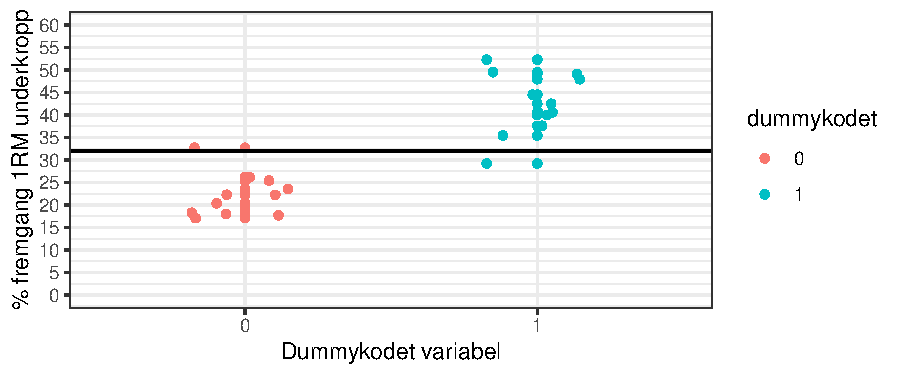
\includegraphics[width=1\linewidth]{04-modellbygging_files/figure-latex/unnamed-chunk-8-1} 

}

\caption{Modeller med forskjellig b1}\label{fig:unnamed-chunk-8}
\end{figure}

\hypertarget{alternativ-modell-alternativ-hypotese}{%
\subsection{Alternativ modell (alternativ hypotese)}\label{alternativ-modell-alternativ-hypotese}}

I forrige avsnitt sa vi at \textbf{null-hypotesen (H0)} reresenterer en en modell som gir samme prediksjon for alle deltakerne som var med i studien uavhengig av hvilken treningsgruppe de tilhører. Vi kalte denne for null-modellen. Vi regnet oss også frem til at denne modellen ga oss en Som of Squared error på 3243.784.

Spørsmålet vi skal stille i dette nå er om vi kan redusere error fra denne ved å benytte en mer kompleks modell som benytter (vår dummykodede kategoriske variabel) som prediktorvariabel:
\[
Y_i = (b_0 + b_1X_i) + error
\]
Prediktorvariabelen b1 er en gruppevariabelen vår som vi dummykodet med tallene 0 og 1.

\[
Fremgang.1RM_i = b_0 + b_1(Gruppe) + error_i
\]
For å holde dette på et overordnet nivå, så vil jeg gi dere de estimerte verdiene for b0 og b1. Målet er å vise dere hvordan denne modellen fungerer. Senere skal gå gjennom hvordan vi regner ut disse verdiene. Trykk her hvis du ønsker å finne ut hvoran du regner ut disse verdiene med en gang.

\[
Fremgang.1RM_i = b_0(21.90) + b_1(20.52*Gruppe) + error_i
\]
Modellen sier at vår b0 er 21.90. Dette er den forventede verdien på Y (Fremgang.1RM) når prediktorvariabelen er 0. Modellen sier også at b1 er 20.52. Med andre ord den forventede økning i Y for en enhets økning i X (også kalt stigningstallet). Husk at vi lagde en gruppe-variabel der vi kodet de to gruppene våre med 0 og 1. Så hvis et individ tilhørte gruppe 0, blir vår prediksjon:

\[
Fremgang.1RM_i = 21.90 + b_1(20.52*0) + error_i
\]
Fordi 0*20.52 = 0, blir stående igjen med b0. Vår prediksjon av et individ som tilhører gruppe 0 blir

\[
Fremgang.1RM_i = 21.90 + 0 + error_i
\]
\[
Fremgang.1RM_i = 21.90 + error_i
\]
Hvis individet derimot tilhører 1 predikerer modellen at individet sin skår blir 42.48.

\[
Fremgang.1RM_i = 21.90 + b1(20.52*1) + error_i
\]
\[
Fremgang.1RM_i = 42.48 + error_i
\]
Visualisert fremstilt blir modellen vår seendes slik ut:

\begin{figure}

{\centering 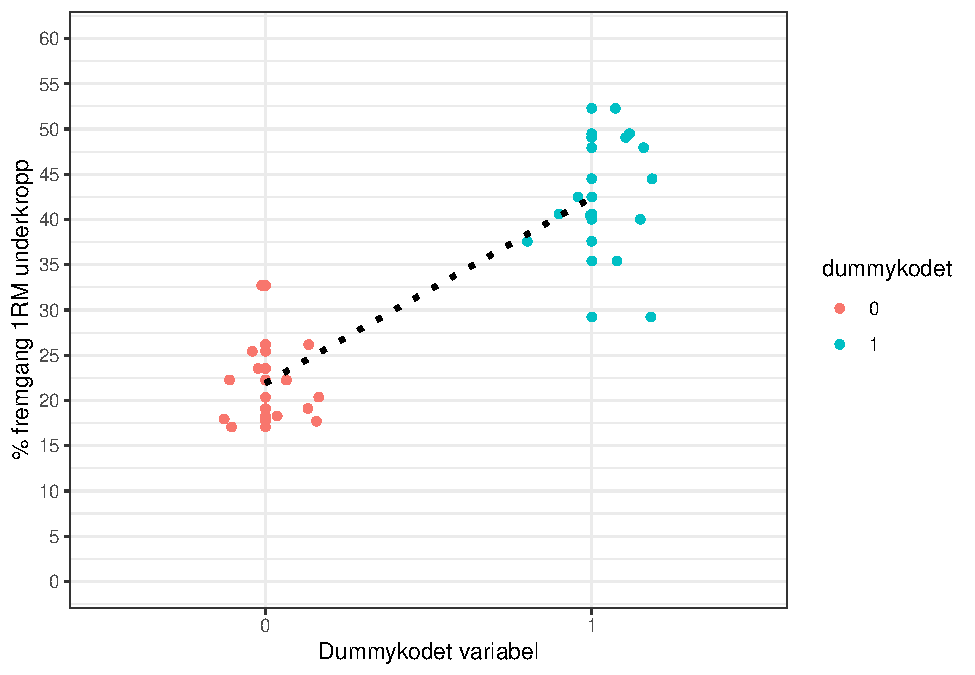
\includegraphics[width=1\linewidth]{04-modellbygging_files/figure-latex/unnamed-chunk-9-1} 

}

\caption{Modeller med forskjellig b1}\label{fig:unnamed-chunk-9}
\end{figure}

\textbf{Oppgave}
Tabellen under viser 6 individer som tilhørte treningsgruppe. Du ser deres faktiske fremgang i 1RM kolonnen. La oss bruke det vi har lært til å predikere disse personene sin fremgang. Vi bruker samme modell som over

\[
Fremgang.1RM_i = b_0(21.90) + b_1(20.52*Gruppe) + error_i
\]
a. Hva predikerer modellen at individ nummer 3 hadde i skår? (to desimaler)

b, Hva hadde individ nr i skår?

\begin{enumerate}
\def\labelenumi{\alph{enumi}.}
\setcounter{enumi}{2}
\tightlist
\item
  hvor mye error blir det?
\end{enumerate}

\begin{enumerate}
\def\labelenumi{\alph{enumi}.}
\setcounter{enumi}{3}
\tightlist
\item
  i Squared Error blir denne erroren?
\end{enumerate}

\begin{enumerate}
\def\labelenumi{\alph{enumi}.}
\setcounter{enumi}{4}
\item
  nå som du har jobbet med denne modellen, så lurer jeg på om det er noe kjent med disse verdiene i modellen. Gå tilbake til {[}link{]} hvis du trenger et hint.
\item
  bo er (norskt ord) for gruppen som er kodet med 0.
\item
  b1 er (norsk ord) mellom gruppen som er kodet med 0 og gruppen som er kodet med 1.
\item
  b0 + b1 er (norsk ord) for gruppen som er kodet med 1.
\end{enumerate}

\begin{table}

\caption{\label{tab:unnamed-chunk-11}Dummy koding}
\centering
\begin{tabular}[t]{r|l|r|r}
\hline
individ & gruppe & rm & dummykodet\\
\hline
1 & tre.sett & 40.467 & 1\\
\hline
2 & tre.sett & 49.072 & 1\\
\hline
3 & tre.sett & 47.941 & 1\\
\hline
4 & tre.sett & 44.514 & 1\\
\hline
5 & tre.sett & 52.288 & 1\\
\hline
6 & tre.sett & 40.018 & 1\\
\hline
\end{tabular}
\end{table}

I forrige oppgave regnet du ut error for ett enkelt individ. Men vi er interessert i den totale erroren for modellen. Formelen for denne er:

total error in den alternative modellen:

SS\_R = \(\sum_{n=1}^N (observert_i - modell_i)^2\)

Med andre ord er det kvadraten av den faktiske observasjonen - hva modellen sa. Bruk formelen til å regne ut dette. (to desimaler

\hypertarget{sammenligne-modeller}{%
\chapter{Sammenligne modeller}\label{sammenligne-modeller}}

Nå som vi har bygget de to statistiske modellene - \textbf{en null-modell} og \textbf{en alternativ modell} - hvor går veien videre? Det vi sitter igjen med er en \textbf{error} (les sum of squared error) for null-modellen og en error for alternative modellen. Vår neste oppgave er å finne en måte å \textbf{sammenligne disse modellene} på. For å gjøre det helt eksplisitt og tydelig, skal vi nå sammenligne om modellen til høyre er bedre enn modellen til venstre.

Når vi sier at en modell er bedre, så mener vi at den vertikale avstanden fra linjen til datapunktene er kort. Hvis det er stor vertikal avstand fra datapunktet til linjen for mange individer, kan det tyde på at vi har en dårlig modell.

\begin{figure}

{\centering \includegraphics[width=1\linewidth]{05-sammenligne_files/figure-latex/unnamed-chunk-2-1} 

}

\caption{Modeller med forskjellig b1}\label{fig:unnamed-chunk-2}
\end{figure}

\hypertarget{anova-tabell-variansanalyse}{%
\section{ANOVA-tabell (variansanalyse)}\label{anova-tabell-variansanalyse}}

En måte vi kan sammenligne modeller på er å bruke en ANOVA-tabell, der vi legger inn erroren vi har regnet for de ulike modellene. Dette er en ganske vanlig tabell som dere kommer til å se flere ganger.

\textbf{ANOVA-tabell}

\begin{longtable}[]{@{}llllll@{}}
\toprule
Modell & SS & \emph{df} & MS & \emph{F} & \(R^2\)\tabularnewline
\midrule
\endhead
The model sum of squares (SSM) & & & & &\tabularnewline
The residual sum of squares (SSR) & & & & &\tabularnewline
The total sum of squares (SST) & & & & &\tabularnewline
\bottomrule
\end{longtable}

{Oppgave}

\begin{enumerate}
\def\labelenumi{\alph{enumi}.}
\tightlist
\item
  Hva er sum of squared error for null-modellen?
\end{enumerate}

Sett dette inn i total sum of squares (SST

\begin{enumerate}
\def\labelenumi{\alph{enumi}.}
\setcounter{enumi}{1}
\tightlist
\item
  Hva er sum of squared error for den alternative modellen?
\end{enumerate}

Sett dette inn i residual sum of squares (SSR). Dette er error som er igjen etter at man har brukt den alternative-modellen. Man kaller dette for \emph{residuals}

\begin{enumerate}
\def\labelenumi{\alph{enumi}.}
\setcounter{enumi}{2}
\tightlist
\item
  Hvor mye sum of squared error er redusert ved å bruke den alternative modellen i forhold null-modellen?
\end{enumerate}

Sett dette inn i residual sum of squares (SSM).Dette kalles The model sum of squares (SSM) eller regression i statistiske programmer. Dere regner dette ved å ta (SST-SSM).

{Godt jobbet!}

Det er ønskelig at SSM er stor fordi det betyr at den alternative modellen vår forklarer mye error. Det kan ofte være lurt å lage figurer for å se dette visuelt. Det er flere måter å gjøre dette på. Vi liker å plotte dette i et stolpediagram, slik vi har gjort i figuren under. På denne måten er det enkelt å se om modellen vår (SSM) er en god eller dårlig modell; hvis høyden på stolpen som representerer SSM er høy betyr det at modellen forklarer mye error. I figuren til venstre ser du modellene vi har bygget, og et eksempel på en modell der SSM er høy. Figuren til høyre er ment som et sammenligningsgrunnlag, der vi viser et eksempel på en dårlig modell.

\begin{figure}

{\centering \includegraphics[width=0.6\linewidth]{05-sammenligne_files/figure-latex/unnamed-chunk-3-1} 

}

\caption{SS for de ulike modellene}\label{fig:unnamed-chunk-3}
\end{figure}

\begin{itemize}
\tightlist
\item
  SST representerer den totale erroren (dvs. erroren vi fikk ved å bruke null-modellen)
\item
  SSR representerer hvor mye error som er igjen etter at vi brukte den alternative modellen.
\item
  SSM er hvor mye error som modellen vår klarte å forklare.
\end{itemize}

\begin{enumerate}
\def\labelenumi{\alph{enumi}.}
\setcounter{enumi}{4}
\tightlist
\item
  Hvis du sammenligner med figuren til venstre (vår modell) med figuren til høyre (som kun er brukt et eksempel), vil du si at vår alternative modell er god?
\end{enumerate}

ja nei.

\begin{enumerate}
\def\labelenumi{\alph{enumi}.}
\setcounter{enumi}{3}
\tightlist
\item
  Hva er (SST) - (SSR)?
\end{enumerate}

\begin{enumerate}
\def\labelenumi{\alph{enumi}.}
\setcounter{enumi}{4}
\tightlist
\item
  Hva er (SSR) + (SSM)?
\end{enumerate}

Med erroren vi har tilgjengelig kan vi regne noe som heter proporsjonal feilreduksjon (proportional reduction in error (PRE)). Hvis vi multipliserer dette tallet med 100 (* 100) får vi hvor mange \% modellen vår har redusert error med, i forhold til null-modellen. Dette er en effektstørrelse som ofte blir rapoortert sammen med ANOVA eller regresjonsanalyser. I ANOVA ser du at man rapporterer denne som \(n^2\), mens man i regresjonsanalyser kaller denne for \(R^2\). Vi regner ut det på følgende måte:

\[
R^2 = \frac{(SS_T - SS_R)}{SS_T} * 100
\]

\begin{enumerate}
\def\labelenumi{\alph{enumi}.}
\setcounter{enumi}{4}
\tightlist
\item
  Hvilken verdi får du hvis du regner (SSM/ (SST)) * 100?
\end{enumerate}

(uten \%-tegnet)

Det er dessverre mange forskjellige navn på denne verdien. Du vil se at folk bruker PRE, \(n^2\). Vit at de mener det samme.

{Ferdig - Bra jobbet!}

\hypertarget{teste-statistisk-om-vuxe5r-alternative-modell-forklarer-mer-varians-enn-null-modellen}{%
\section{Teste (statistisk) om vår alternative modell forklarer mer varians enn null-modellen}\label{teste-statistisk-om-vuxe5r-alternative-modell-forklarer-mer-varians-enn-null-modellen}}

En error-reduksjon på 2527.5 (\(SS_M\)), eller 78 \% (\((R^2)*100\)), kan høres mye ut. Men et problem med disse størrelsene er at de begge er garantert å øke i takt med antall parametere vi legger til i modellen. Dere har ikke lært dette enda, men vit at vi kunne bygget en modell der vi inkluderer kjønn, alder, treningsstatus som prediktorvariabler. Da ville dere fått en mer kompleks modell:

\[
Y_i  = b_0 + b_1(Gruppe_i) + b_2(Kjønn_i) + b_3(Treningstatus_i) + b_4(Alder_i)
\]

Hvis vi hadde gjort dette, ville vi fått en høy \(SS_M\) eller \(R^2\). Derfor er det mer interessant å regne ut gjennomsnittlig \(SS_M\) per parameter vi har lagt til i modellen (i forhold til null-modellen). Dette kalles \textbf{Mean Squared Model (MSM)}, eller gjennomsnittlig squared error for den alternative modellen, og regnes på følgende måte:

\[
\text{ Mean Squared Model } (MS_M) = SS_M / df_M
\]
\(df_m\) står for antall frihetsgrader som er lagt til i modellen utover null-modellen. Null-modellen har kun ett parameter (\(b_0\)), som er mean, mens vår alternative modell har to parametere (\(b_0\) og \(b_1\)). Derfor blir \(df_M\) = (2-1) = 1.

\begin{enumerate}
\def\labelenumi{\alph{enumi}.}
\tightlist
\item
  Regn ut Mean Squared Error (\(MS_M\)) og sett det verdien inn i ANOVA-tabellen vår
\end{enumerate}

\textbf{ANOVA-tabell}

\begin{longtable}[]{@{}llllll@{}}
\toprule
Modell & SS & \emph{df} & MS & \emph{F} & \(R^2\)\tabularnewline
\midrule
\endhead
The model sum of squares (SSM) & 2527.5 & & & & 0.78\tabularnewline
The residual sum of squares (SSR) & 716.2875 & & & &\tabularnewline
The total sum of squares (SST) & 3243.784 & & & &\tabularnewline
\bottomrule
\end{longtable}

Det vi ønsker at dere tar med dere fra denne oppgaven er at en høy \(SS_M\) eller \(R^2\) er \textbf{mer imponerende hvis vi kun har lagt til ett ekstra parameter enn hvis vi hadde lagt til f.eks. 10 parametere}. Enig?

{Bra!}

Det siste vi skal gjøre er å sammenligne \(MS_M\) med \(MS_R\). \textbf{\(MS_R\)} er \(SS_R\), den erroren som er igjen etter at vi har brukt den alternative modellen, \textbf{delt på antall parametere som i prinsippet kunne vill lagt til i modellen}. I prinsippet står vi fritt til å legge til så mange parametere i modellen som vi ønsker, men antall parametere kan aldri overstige antall deltakere i studien. Men fordi vi allerede har brukt to parametere i den alternative modellen, kan vi kun legge til (24 - 2) = 22 parametere.

\[
\text{ Mean Squared Residual (MSR) }  = SS_R / df_R
\]
b. Regn ut Mean Squared Residual (\(MS_R\)) og sett det verdien inn i ANOVA-tabellen vår

\textbf{ANOVA-tabell}

\begin{longtable}[]{@{}llllll@{}}
\toprule
Modell & SS & \emph{df} & MS & \emph{F} & \(R^2\)\tabularnewline
\midrule
\endhead
The model sum of squares (SSM) & 2527.5 & & 2527.5 & & 0.78\tabularnewline
The residual sum of squares (SSR) & 716.2875 & & & &\tabularnewline
The total sum of squares (SST) & 3243.784 & & & &\tabularnewline
\bottomrule
\end{longtable}

\(MS_R\) er gjenstående error per parameter som potensielt kunne blitt lagt til i modellen. Med andre ord er det den gjennomsnittlige erroren som er igjen per parameter som kunne blitt lagt til i modellen. Enig?

{Vi er endelig i mål!}

Nå har vi gjort alle utregningene, og vi kan bare sammenligne disse to størrelsene (\(MS_M\) versus \(MS_R\)) med hverandre. Dette kalles en \textbf{F-test}.

\[
\text{F}  = \frac{MS_M}{MS_R}
\]

\begin{enumerate}
\def\labelenumi{\alph{enumi}.}
\setcounter{enumi}{2}
\tightlist
\item
  Regn ut vår F-verdi og sett den inn i vår ANOVA-tabell
\end{enumerate}

\textbf{ANOVA-tabell}

\begin{longtable}[]{@{}llllll@{}}
\toprule
Modell & SS & \emph{df} & MS & \emph{F} & \(R^2\)\tabularnewline
\midrule
\endhead
The model sum of squares (SSM) & 2527.5 & 1 & 2527.5 & & 0.78\tabularnewline
The residual sum of squares (SSR) & 716.2875 & 22 & 32.55852 & &\tabularnewline
The total sum of squares (SST) & 3243.784 & & & &\tabularnewline
\bottomrule
\end{longtable}

Vi kan se at vår F-verdi er 77.63, og at p-verdien er \textless{} 0.001. Denne verdien (vises kke i figuren under pga. størrelsen) er høyere enn vår kritiske verdi (den røde streken) for 0.05 ved \(df_M\) = 1 og \(df_R\) = 22. Vi sier derfor at vår modell er signifikant, hvilket vil si at den har forbedret vår evne til å predikere utfallsvariabelen. En F-fordeling ser veldig lik ut som en z- og t-fordeling, og fungerer på samme måte: Vi regner ut en F-verdi, og spør om sannsynligheten for å oppnå en slik verdi gitt at null-hypotesen er sann. Null-hypotesen i en F-test er at den alternative modellen ikke forklarer noe varians. Med andre ord at \(R^2\) = 0.

\begin{figure}

{\centering \includegraphics[width=0.6\linewidth]{05-sammenligne_files/figure-latex/unnamed-chunk-4-1} 

}

\caption{F-test}\label{fig:unnamed-chunk-4}
\end{figure}

{Done!}

Da er det bare å sette seg tilbake å nyte denne sangen:

\begin{figure}
\centering
\includegraphics{F.png}
\caption{F-testen}
\end{figure}

Hvis dette ikke var forståelig foreslår jeg følgende tutorials:
- \url{https://www.youtube.com/watch?v=eSJAjlavPwU}
- \url{https://www.youtube.com/watch?v=0xWDulRHd9M}
- \url{https://www.youtube.com/watch?v=iAE4UeoVE9A}
- \url{https://www.youtube.com/watch?v=OK4Xns4zabs}

\begin{Shaded}
\begin{Highlighting}[]
\CommentTok{\#aov er en forkortolse for analysis of variance (ANOVA)}
\CommentTok{\#dette er funksjon som kommer mer R.}
\FunctionTok{summary}\NormalTok{(}\FunctionTok{aov}\NormalTok{(rm }\SpecialCharTok{\textasciitilde{}}\NormalTok{ dummykodet, dat))}
\end{Highlighting}
\end{Shaded}

\begin{verbatim}
##             Df Sum Sq Mean Sq F value   Pr(>F)    
## dummykodet   1 2527.5  2527.5   77.63 1.15e-08 ***
## Residuals   22  716.3    32.6                     
## ---
## Signif. codes:  0 '***' 0.001 '**' 0.01 '*' 0.05 '.' 0.1 ' ' 1
\end{verbatim}

\hypertarget{hvordan-finne-linjen-i-modellen}{%
\chapter{Hvordan finne linjen i modellen?}\label{hvordan-finne-linjen-i-modellen}}

Nå som vi er kjent med hvordan vi kan bygge og teste statistiske modeller, er det på tide å vise hvordan vi finner regresjonslinjen som vi skal bruke. Mer presist, hvilke verdier skal vi ha for \emph{b}0 og \emph{b}1 som beskriver denne linjen? Hittil har dere fått disse verdiene av meg, men det vi skal lære nå er hvordan vi kan regne ut disse verdiene for hånd. En viktig sannhet om denne linjen er at regresjonslinjen (les modellen) er plassert slik at den reduserer Sum of Squared Error mest mulig. Med andre ord, verdiene på \emph{b}0 og \emph{b}1 (som beskriver denne linjen) er slik at det er umulig å redusere error mer. Spørsmålet er hvordan vi finner verdiene på \emph{b}0 og \emph{b}1 som beskriver denne linjen. En tilnærming kan være å gjette seg fram til hva \(b_0\) og \(b_1\) skal være. Vi kan teste ut ulike verdier for b0 og b1, og evaluere hvor mye sum of Squared Error disse gir. I figuren under har jeg prøvd tre ulike modeller, og regner ut hvor mye sum of squared error disse gir.

\begin{figure}

{\centering \includegraphics[width=0.8\linewidth]{06-linje_files/figure-latex/unnamed-chunk-1-1} 

}

\caption{Ulike linjer}\label{fig:unnamed-chunk-1}
\end{figure}

{Oppgave}

\begin{enumerate}
\def\labelenumi{\alph{enumi})}
\tightlist
\item
  Hvilken av modellene over gir mest sum of squared error? (SSModel)
\end{enumerate}

b0=30 b1=7 b0=25 b1=28 b0=10 b1=30

Vi kan holde på slik med slik prøving-og-feiling til vi faktisk finner linjen som reduserer error mest. Det er bare å teste nok verdier. \textbf{Minste kvadraters metode} garanterer oss å alltid gi oss er svar. Jeg har laget en video til dere som viser vi kan prøve-og-feile til vi kommer frem til en løsning (se denne):

Det er en mer effektiv måte å løse dette problemet på. For å finne \textbf{b1} kan vi bruke følgende formel:

\[ b_1 = \frac{SCP}{SS_x} \]
Her var det et nytt begrep, \textbf{SCP}. SCP står for sum of cross-product deviations. Det brukes til å finne relasjonen mellom to variabler, og er grunnlaget for en rekke utregninger i statistikken, så det kan være lurt å lære seg. SCP finner ut av om en person som er over eller under gjennomsnittet på en variabel, også er over eller under gjennomsnittet på den andre variabelen.

\[ b_1 = \frac{SCP = \sum_{n=1}^N (x_i - \bar{x})(y_i - \bar{y})}{SS_x} \]
\(\bar{x}\) er gjennomsnittet på x-variabelen (gruppe), mens \(\bar{y}\) er gjennomsnittet for y-variabelen (1RM). I tabellen under ser du hvordan vi regner dette. Kolonnen CrossProduct er \((x_i - \bar{x})(y_i - \bar{y})\).

\begin{table}

\caption{\label{tab:unnamed-chunk-2}Utregning av Sum of Cross Product (SCP)}
\centering
\begin{tabular}[t]{rrrrrrrr}
\toprule
individ & gruppe & gj.snitt.x & error.x & rm & gj.snitt.y & error.y & CrossProduct\\
\midrule
1 & 1 & 0.5 & 0.5 & 40.46704 & 32.16231 & 8.3047301 & 4.1523651\\
2 & 1 & 0.5 & 0.5 & 49.07223 & 32.16231 & 16.9099106 & 8.4549553\\
3 & 1 & 0.5 & 0.5 & 47.94131 & 32.16231 & 15.7789994 & 7.8894997\\
4 & 1 & 0.5 & 0.5 & 44.51389 & 32.16231 & 12.3515740 & 6.1757870\\
5 & 1 & 0.5 & 0.5 & 52.28750 & 32.16231 & 20.1251864 & 10.0625932\\
\addlinespace
6 & 1 & 0.5 & 0.5 & 40.01750 & 32.16231 & 7.8551872 & 3.9275936\\
7 & 1 & 0.5 & 0.5 & 49.48425 & 32.16231 & 17.3219362 & 8.6609681\\
8 & 1 & 0.5 & 0.5 & 29.21048 & 32.16231 & -2.9518368 & -1.4759184\\
9 & 1 & 0.5 & 0.5 & 40.59293 & 32.16231 & 8.4306117 & 4.2153059\\
10 & 1 & 0.5 & 0.5 & 37.58676 & 32.16231 & 5.4244472 & 2.7122236\\
\addlinespace
11 & 1 & 0.5 & 0.5 & 35.42651 & 32.16231 & 3.2641906 & 1.6320953\\
12 & 1 & 0.5 & 0.5 & 42.49354 & 32.16231 & 10.3312265 & 5.1656133\\
13 & 0 & 0.5 & -0.5 & 17.70576 & 32.16231 & -14.4565510 & 7.2282755\\
14 & 0 & 0.5 & -0.5 & 17.07181 & 32.16231 & -15.0905068 & 7.5452534\\
15 & 0 & 0.5 & -0.5 & 18.26811 & 32.16231 & -13.8942055 & 6.9471027\\
\addlinespace
16 & 0 & 0.5 & -0.5 & 25.42594 & 32.16231 & -6.7363771 & 3.3681886\\
17 & 0 & 0.5 & -0.5 & 32.70313 & 32.16231 & 0.5408147 & -0.2704074\\
18 & 0 & 0.5 & -0.5 & 19.10226 & 32.16231 & -13.0600552 & 6.5300276\\
19 & 0 & 0.5 & -0.5 & 22.23827 & 32.16231 & -9.9240435 & 4.9620217\\
20 & 0 & 0.5 & -0.5 & 22.27148 & 32.16231 & -9.8908322 & 4.9454161\\
\addlinespace
21 & 0 & 0.5 & -0.5 & 26.17889 & 32.16231 & -5.9834246 & 2.9917123\\
22 & 0 & 0.5 & -0.5 & 20.34857 & 32.16231 & -11.8137453 & 5.9068726\\
23 & 0 & 0.5 & -0.5 & 23.52773 & 32.16231 & -8.6345853 & 4.3172926\\
24 & 0 & 0.5 & -0.5 & 17.95966 & 32.16231 & -14.2026514 & 7.1013257\\
\bottomrule
\end{tabular}
\end{table}

\[ b_1 = \frac{SCP = 20.52436}{SSx} \]
Nå som vi har regnet SCP er det bare å regne SSx (sum of squared error for prediktorvariabelen) er fordi man ønsker å ta høyde for hvor mye prediktorvariabelen avviker fra mean. Jeg har dessverre ikke noen supergod forklaring, og jeg synes heller ikke Field forklarer dette godt. Så jeg bare vet at jeg må gjøre det.

\[ b_1 = \frac{SCP = 20.52436}{6} \]
\[ b_1 = 20.52436 \]

Nå gjenstår det bare å finne \textbf{b\_0}. Denne er enkel å finne når vi først har funnet \textbf{b0}. Husk at modellen vår er en ligning, så ved enkelt finne \textbf{b0} ved omorganisere ligningen: trekker vi fra \(b_1X_i\) på hver side av likhetstegnet får vi \textbf{b0} alene:

\[
Y_i = (b_0 + b_1X_i)
\]

\[
Y_i - b_1X_i = (b_0)
\]

Men må ligningen med verdier. Og da bruker man gjennomsnittet for Y variabelen og gjennomsnittet for X variabelen.

\[
32.16231     - (20.52436*0.5) = (21.90013)
\]

\hypertarget{t-test---er-b_1-signifikant-forskjellig-fra-null}{%
\chapter{\texorpdfstring{T-test - er \(b_1\) signifikant forskjellig fra null?}{T-test - er b\_1 signifikant forskjellig fra null?}}\label{t-test---er-b_1-signifikant-forskjellig-fra-null}}

En F-test tester om vår alternative modell er en bedre modell enn null-modellen, totalsett. Men det kanskje mest interessante spørsmålet er fremdeles er fremdeles delvis ubesvart:
* \textbf{er b1 i modellen vår, altså vårt stigningstall som representer den forventede endringen i utfallet for en enhets endring i prediktorvariablen, signifikant forskjellig fra null?}

Før du leser videre, forsøk å forestill deg hvordan en modell med en b1 som er 0 ser ut? Deretter se på figurene under

\begin{itemize}
\tightlist
\item
  Hvis b1 er 0, er det ingen relasjon mellom disse prediktorvariabelen (x) og utfallsvariabelen (y).
\item
  Hvis b1 er \textgreater{} enn 0, er det en positiv relasjon mellom vår prediktovariabel og utfallsvariabelen.
\item
  Hvis b1 er \textless{} enn 0, er det en positiv relasjon mellom vår prediktovariabel og utfallsvariabelen.
\end{itemize}

Husk at b1 i vårt tilfelle representer forskjellene i gjennomsnitt mellom de to gruppene. Det er med andre ord like gyldig å spørre om det er en relasjon mellom variablene som at det er en forskjell i means mellom to grupper.

Vi kan tydelig se at b1 er forskjellig fra 0 i vårt utvalg, men husk at denne forskjellen kan skyldes sampling variation som vi kan forvente under null-hypotesen. Vi må derfor teste om de to utvalgene vi har kommer fra samme eller to forskjellige populasjoner (en endring som i så fall har skjedd fordi vi har gitt de to utvalgene forskjellig treningsopplegg). Dette kan vi finne ut ved å kjøre en uavhengig t-test.

\[
t.test = \frac{(b_1observert - b_1forventet)}{\text{standard error of } b_1}
\]
Vi vet allerede b1observert (den observerte forskjellen mellom de to utvalgene) og b1forventet (null-hypotesen er at det ikke er noen relasjon mellom disse variablene, så denne blir null. Så vi kan plotte inn disse verdiene.

\[
t.test = \frac{(20.52 - 0)}{\text{standard error of } b_1}
\]
Det som gjenstår er å finne ut hva standard error of b1 er. Vi har tidligere regnet ut standard error of mean \(SD/sqrt(N)\), og vi kan gjøre noe lignende for å regne ut standard error of b1. Men for å fokusere på det store bildet vil jeg gi dere den estimerte standard error of b1

Prosedyren for å regne ut standard error of b1 er ikke vanskelig, men det er en del utregningsledd. Så lenge dere forstå at standard error of b1 er et mål på hvor mye utvalg vil være forskjellige fra hverandre, så tenker jeg at dere ikke vil øke deres forståelse ved å lære å regne standard error of b1, men jeg kan selvfølgelig ta feil. Jeg anbefaler dere på det sterkeste at der ser \href{https://www.youtube.com/watch?v=3L9ZMdzJyyI}{denne videoen}

Fra mitt output i Jamovi kan jeg lese at standard error of b1 er \textbf{2.33}.

\begin{figure}
\centering
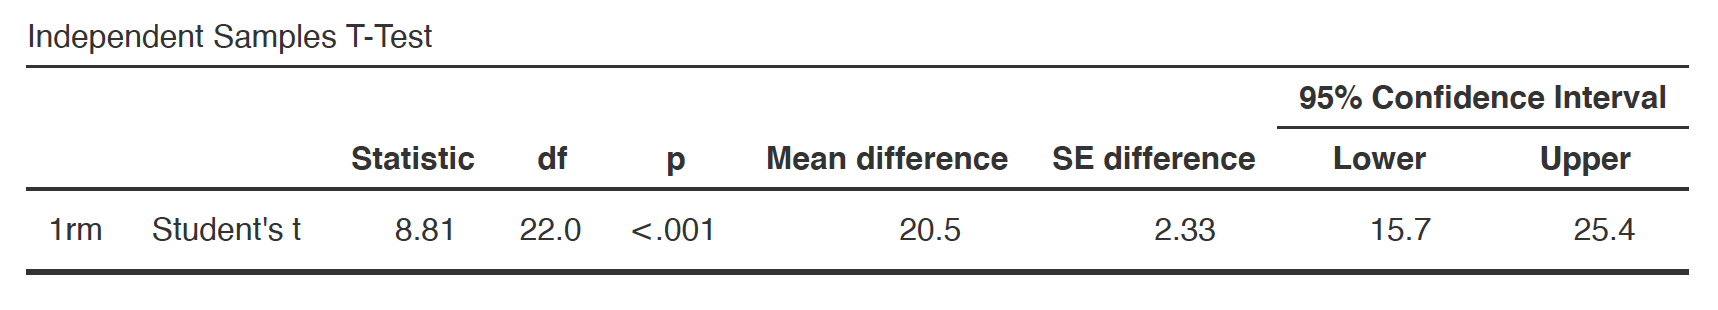
\includegraphics{output.png}
\caption{ny}
\end{figure}

Så jeg kan bruke dette i utregningen av t.

\[
t.test = \frac{(20.52 - 0)}{2.33}
\]

\[
t.test = \frac{(20.52 - 0)}{\text{standard error of } b_1}
\]
\[
t.test = 8.806867
\]
Vår t-verdi er 8.80. Vi kqn se tydelig se at denne t-verdier er større enn den kritiske verdien på \textasciitilde{} 2, så vi kan konkludere at vi har et signifikant funn; ee to utvalgene vi har med i studien synes å komme fra forskjellig populasjon. Vi kan lese denne t-verdien fra output tabellen fra Jamovi at vår p-verdi er \textless{} 0.001.

En liten notis som er viktig å være observant på.

\begin{figure}

{\centering \includegraphics[width=1\linewidth]{07-ttest_files/figure-latex/unnamed-chunk-1-1} 

}

\caption{t-fordelingen og vår t-verdi}\label{fig:unnamed-chunk-1}
\end{figure}

\hypertarget{write-up}{%
\chapter{Write-up}\label{write-up}}

Det er en ganske standardiser måte å rapporte en statistisk test på. Først skriver du hva har testet. Husk at du bare har gitt statistikprogrammet noen tall og fått et resultat. Nå må du kommunisere til andre.

'Deltakerne i 1L-3U 3L-1U-gruppen hadde i gjennomsnitt mindre større en lavere \% fremgang 1RM, på underkroppsøvelser (M=,SD=), enn som {[}{]}. Denne forskjellen, {[}{]}, CI {[}{]}, var signifikant, \emph{t}({[}{]}) = {[}{]}, p = {[}{]}, d={[}{]}.

\hypertarget{visualisering-av-ulike-statistiske-modeller-1}{%
\chapter{Visualisering av ulike statistiske modeller}\label{visualisering-av-ulike-statistiske-modeller-1}}

{Modeller med samme b0, men forskjellig b1}

I figurene under ser tre ulike modeller med uinteressante X og Y variabler. Alle har samme b0, mens de har forskjellig b1. Husk at b1 forteller om relasjonen mellom X og Y.

\begin{itemize}
\item
  I \textbf{modell A} ser du at når X øker, øker Y med 0.4 \textbf{for hver enhets økning i X}.
\item
  I \textbf{modell B} er det ingen relasjon mellom X og Y, så for en enhets økning i X, vil vi forvente at Y forblir den samme.
\item
  I \textbf{modell C} er det en negativ relasjon mellom X og Y. Denne modellen sier at for en enhets økning i X, vil vi forvente at Y går ned med 0.4 (siden den er negativ).
\end{itemize}

\begin{figure}

{\centering \includegraphics[width=1\linewidth]{forelesning_files/figure-latex/unnamed-chunk-1-1} 

}

\caption{Modeller med forskjellig b1}\label{fig:unnamed-chunk-1}
\end{figure}

{Modeller med forskjellig b1, men samme b1}

\begin{figure}

{\centering \includegraphics[width=1\linewidth]{forelesning_files/figure-latex/unnamed-chunk-2-1} 

}

\caption{Modeller med forskjellig b0}\label{fig:unnamed-chunk-2}
\end{figure}

{Hva blir vår modell?}

\begin{figure}

{\centering \includegraphics[width=1\linewidth]{forelesning_files/figure-latex/unnamed-chunk-3-1} 

}

\caption{Vår data}\label{fig:unnamed-chunk-3}
\end{figure}

  \bibliography{book.bib,packages.bib}

\end{document}
